\graphicspath{{chapters/10/images/}}
\chapter{Least squares problems}


Recall that if $m$ is the model, we quantified the distance between the
model output and data as:

$$
m_j(t_i,(x_0,t_0), \theta) = m_{ij}(\theta) - \hat{y}_{ij}, \text{for } i,j \text{ as lesson 2 }
$$

$r_{ij}(\theta)$ is called RESIDUAL and we shape it as a vector.

$$
J_k=J(\theta_k)[\frac{\partial r_I}{\partial\theta_i}], i=1, ...,n, I=1,...n
$$
\\
\\
\noindent
Since the time points are given by the data, everything only depends on
the choice of parameter theta, which is a vector of parameters. We can
derive the residual according to theta. Our function to minimize is
$f(\theta)=\frac{1}{2}\sum^m_{j=1}r_j^2(\theta)$
\noindent
It will hardly go to zero, as our observations are affected by noise: we
just need to explain data, not noise. If we have the distance of the
single point we can see the effect of each parameter by looking at the
derivative. Here we have that the gradient (Jacobian) will be telling us
the relationship among model parameters and data.

$$
\nabla f(\theta)=\sum^m_{j=1}r_j(\theta)\nabla r_j(\theta)= J(\theta)^Tr(\theta)
$$
\noindent
The matrix notation is a more convenient way to express this gradient.
While solving least squares problems we always exploit Taylor
approximation.

Hessian matrix:

$$
\nabla^2 f(\theta)=J^T(\theta)J(\theta)+ \sum^m_{j=1}r_j(\theta) \nabla^2 r_j(\theta)
$$
\noindent
What's \emph{magical} of this is that we can use $J^T(\theta)J(\theta)$
as approximation for $B(\theta)$ of our gradient.

If the problem is linear, $r(\theta)=A(\theta)-y$. The objective
function $f(\theta)=\frac{1}{2} || A\theta-y||^2$ and
$\nabla f(\theta)=A^T(A\theta-y), \nabla^2 f(\theta)=A^TA$.

If $f$ is convex
$\Rightarrow \exists \theta^* s.t. \nabla f(\theta^*)=0 - A^TA\theta^*=A^Ty$
\\
\\
\noindent
We reach a normal equation, linear system (we know how to solve this). With general functions, this is not so straightforward; what we will do
is approximating the problem with a solvable linear problem.
\\
\\
\noindent
When we try to quantify the distance between the model and our points we can formalize the problem as:

$$
r_i = m_i(t,\theta) - y_0 \\ f(\theta)= \frac{1}{2} \sum^m_{j=1} r_j^2 (\theta) \\ \nabla f(\theta) = J(\theta)^{T} r (\theta) \\ \nabla f(\theta) = J(\theta)^{T} J (\theta) + \sum^m_{j=1} r_j \theta \nabla^2 r_3 \theta\\
$$
\noindent
Last time we already said that we will ignore the sum, for two reasons:

\begin{enumerate}
\def\labelenumi{\arabic{enumi}.}
\tightlist
\item
  it contains second order derivatives, painful to compute
\item
  the Newton direction is a quasi vector
\end{enumerate}

So at every iteration $k$ we solve the approximated problem

$$
J(\theta_k)^TJ(\theta_k)p=-J(\theta_k)r(\theta_k) \\ J_k^TJ_kp=-J_k^T r_k
$$
\noindent
This is a linear system which we can solve. In this case, we are
solving:

$$
f(\theta_k+p)= \frac{1}{2} ||r(\theta_k+p)||^2 \simeq \frac{1}{2} ||J_kp+r_k||^2
$$
\noindent
This is what we called normal equation for a normal least squares
problem. Under certain hypotheses the method converges quadratically!
\\
\\
\noindent
We discussed last time that Newton is quadratic convergent. Of course
the matrix should not be singular, we need to be able to solve the
system. We start with a problem in a special form, sum of squares.
Thanks to this, we can rewrite the problem in a simpler way and perform
an approximation, leading to solving a linear system at each iteration.
This approximation guides us rapidly to a solution. We are applying
linear search, by defining a direction and solving a new problem at each
iteration. The biggest issue could be the non invertible matrix, but we
can do something to circumvent the issue.


\subsection{The Levenberg-Marquardt method}

At each iteration, we solve the problem:

$$
\min_{||p||\leq\delta_k} \frac{1}{2} ||J_kp-r_k||^2
$$
\noindent
We can have a solution inside the trust region $\delta_k$ or on the
border i.e.~not the minimum, but the smallest value we can reach.

\begin{itemize}
\item
  case 1: $\beta$ is a solution and $||p||\leq\delta_k$ → DONE
\item
  case 2: $||p||=\delta_k$ , then $\bar{p}$ is a solution if and only if
  $\exists \lambda > 0$:

  $$
    (J^TJ-\lambda I)=-J^Tr \\ + \lambda(\delta_k-||p||)=0
    $$
\end{itemize}
\noindent
If we can push it a bit further from zero and the problem is still
solved, we can think of it as a solution. If we are hitting the boundary
$\lambda(\delta_k-||p||)=0$, we want to move the matrix a bit from
singularity. We will not use it very much, but it is a well known
algorithm. It is one of the default MATLAB solvers. The
Levenberg-Marquardt converges quadratically when we are close to the
solution, while if the residuals are big it does not perform well.


\subsection{Solving a problem with bounds}
We have seen together that we can exploit the Lagrangian for the
  equality constraint, but we can have other boundaries. There are other
  approaches which allow us not to lose our approximation advantage. We
  can simply do \textbf{\emph{variable transformation}} : instead of
  changing the problem, we change the variables.
\noindent
Example: $x \rightarrow e^x, \mathbb{R} \rightarrow \mathbb{R}_0^?$
{[}other example missing, cannot understand from recording{]}
\\
\\
\noindent
 Another solution could be to include the bound in the \textbf{\emph{trust region}}.

{[}drawing missing{]}
\noindent
\emph{Evolutionary algorithms} follow the evolution of the solution: at
the beginning look for solutions, then add a penalty for the boundaries.

\subsection{Solving global minimum problem}

How can we be sure that we are looking at a global minimum? We can start
from another initial point and check whether the solution reaches the
same minimum.
\noindent
From local to global → the \textbf{\emph{multi-start approach,}} t is a
shortcut, but the best way to work.

\subsection{Gauss-Newton method}

Let $N \in \mathbb{N}, \varepsilon > 0, J$ as defined before. We randomly select N vectors and use
$\theta^1, \dots, \theta^n \in \mathbb{R}^n$

For each $i=1,\dots,N$ DO

REPEAT

$\bar{J}=J(\theta^i)$

compute $q$ s.t. $\bar{J}^i\bar{J}q=-\bar{J}r(\theta^i)$

compute $\vartheta = \theta^i + q$

compute $\varepsilon = ||\frac{\theta^i-\vartheta}{\theta}||$,
\emph{relative increase}

update $\theta^i = \vartheta$

IF $\varepsilon<\bar{\varepsilon}$ then BREAK

SAVE $\theta^i$

END

→ no global minimum guarantee!
\\
\\
\noindent
There are other ways to detect if a minimum is global e.g.~we try to
divide the space in N different sectors and pick points for each one of
them, \emph{Latin hypercube} and \emph{orthogonal sampling}. The more we
do it, the more we acquire confidence, but we will never be sure. In
addition, we always have to deal with noise, we do not know if the
minimum is the best or we are overfitting.
\\
\\
\noindent
Example on MATLAB: if we take only 10 random points we can have a biased
result. By taking a bigger sample, we should somehow achieve a fuller
result in the region. Still, we have some holes and repeated points. Are
there smarter ways to take random points?


\subsection{Latin hypercube sample}

Get random numbers dividing the interval in m sectors. This is a 2x2
problem and we need to reason on some aspects: if we take the square
(0,1),(0,1) out of 100 points we will just have 3/4 there → not
exploring it very well. If parameters are between 0.1 to 1000 we need to
better sample.

$n = 20$, the fewer points we get, the more we see the difference among
the two methods.

$n = 200$, still we have missing parts.

$n = 2000$, thousands of iterations → if we zoom in there is still a lot
of space
\\
\\
\noindent
The takehome message is that it is almost impossible to cover all the
space with points. Luckily these are starting points, if they are close
to the solution we will have the good direction. Gradient methods are
expensive, but they are smart.


\subsection{MATLAB}

When an optimizer stops, it gives as output the function converged to
the solution or why it stopped. Termination criteria: gradient,
incremental step e.g.~is our step too small?, change in x was less of
certain tolerance, the residual was less than specific tolerance, max
number of iterations. These conditions are added in order to avoid
infinite function evaluation.
\\
\\
\noindent
We first need to define an enzymatic reaction as a set of ODEs. We then
specify initial concentrations and a given set of rates. Integrate the
model and plot the simulation results.
\\
\\
\noindent
The dots are the experimental points, lines are the output of the
simulation. According to different starting points, we will obtain
different results; we need to quantify how much the model is distant
from the real data. The output of the normal simulation is a set of
points; we can do a linear interpolation for time and values, giving how
much is each of the simulated variables at the requested time. Once we
have the values at the right time, we can compute the \emph{residuals}
through the sum of squares. In some cases we can also look at weighted
residuals and normalize them; however, zeros are problematic → our
experimental data goes to zero, we stick to normal SSE.
\\
\\
\noindent
Our objective function takes the rate, experimental time and values,
initial and final time. We call the solver (15s as the system is stiff,
we require a more robust iteration) and get a vector of residuals and
SSE.
\\
\\
\noindent
If we compute the residual with $s_1$,$s_2$ and $s_3$ we can easily understand
which is the better one (matches visual inspection of the plot).
\\
\\
\noindent
We can then optimize and find the solution with \texttt{lsqnonlin}
e.g.~$SSE1 = 33.6653$, $resNorm = 38$, worse, we should improve initial
conditions.

{[}Recap from last time{]}
\\
\\
\noindent
\textbf{MATLAB multi-start} is a wrapper working with different
algorithms. It will automatically parallelize the problem. It requires
to insert starting points and tolerance. We therefore define bound,
create problem and give initial points e.g.~lsqnonlin + objective
function. The output contains the result of parallel lsqnonlin and
parameters, somehow similar to what we saw before. We can reduce the
bounds, but solution 1 is still the best. Main limitation: heavily
depends on the number of initial points.

\begin{figure}
\centering
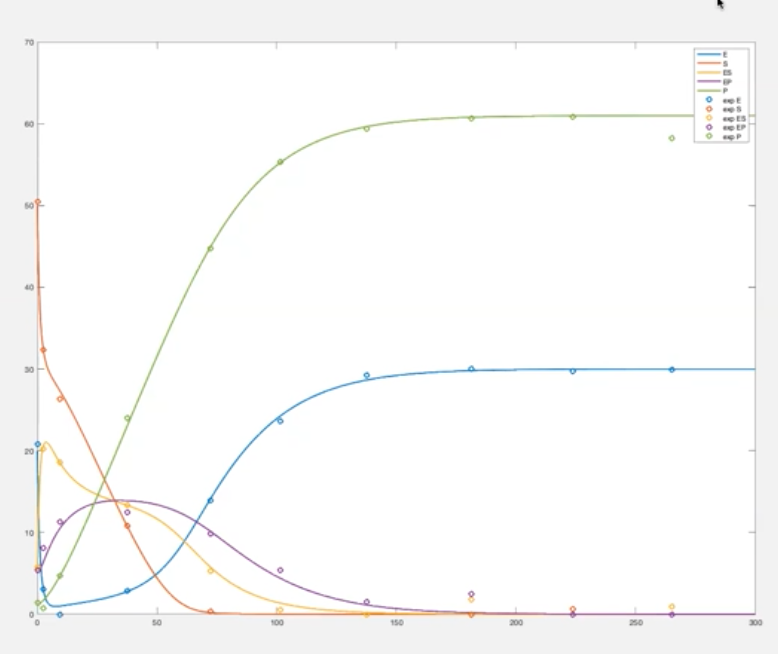
\includegraphics[width=0.45\textwidth]{multistep.png}
\caption{MATLAB multi-start lsqnonlin}
\end{figure}

\noindent
Remarks:

\begin{itemize}
\tightlist
\item
  we did a lot of computations
\item
  $s_1$, the initial set of parameters, had values at different orders
  of magnitude. We really do not know if we are doing well or not.
\end{itemize}
